\chapter{Additional Developed Software} \label{chap:othersoft}


\section{\texttt{TDB-Highlighter}} \label{osoft:sec:tdbhighlighter}

\hspace{24pt} Motto: \textit{You didn't know you can't do CALPHAD without it.}

This VS Code Language Extension, developed from scratch by Adam M. Krajewski, provides syntax highlighting for the Thermodynamic DataBase (\texttt{TDB}) files used in the CALPHAD community to describe thermodynamic properties of materials. 

As of June 2024, it was installed by 173 users of VS Code and holds 5/5 stars rating in the VS Code Marketplace under \href{https://marketplace.visualstudio.com/items?itemName=amkrajewski.tdb-highlighter#review-details}{AMKrajewski.tdb-highlighter} software identifier.

\textbf{Most critically, if something is highlighted differently than you expect, you know something may be wrong with it}. E.g., in \texttt{+1.95033E-07*T**3-.01798O876*T**2+78.5244752*T*LN(T)-722.59722*T+229382.886-93813648*T**(-1); 3290 Y} one of the numbers is not a number and will be red. One can guess which one... Likewise, that \texttt{LAVE\_C36} phase one just typed will stand out.

Features include:
\begin{itemize}
    \item Phases, species, elements and other critical elements of the database, are formatted with highly visible fonts and colors, speeding up the process of navigating, reading, and editing the files tremendously.
    \item References, notes, comments, optionals, and otherwise less critical parts of the database, are formatted with subtle formatting to reduce visual clutter.
    \item Temperature (T) and its powers/logs/exps in equations are formatted with bright red colors to immediately pinpoint where a given part of the polynomial is located.
    \item Function names are exposed within the equations to make them stand out from numbers and be easier to read.
    \item A number of TDB syntax keywords are specifically highlighted in neutral colors matching their functions to make them stand out in case of typos.
\end{itemize}

Together, they yield the following neat-looking TDB header shown in Figure~\ref{osoft:fig:tdbheader}.

\begin{figure}[H]
    \centering
    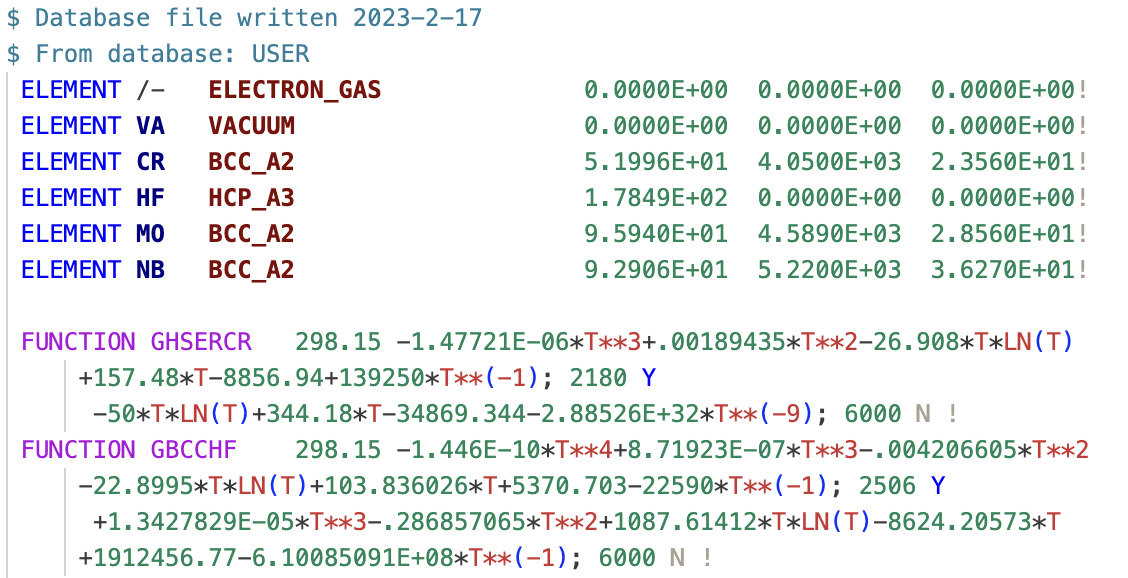
\includegraphics[width=0.65\textwidth]{tangentialsoft/Fig1.png}
    \caption{Header of am example TDB file (including some function definitions) syntax-highlighted using \texttt{TDB-Highlighter}.}
    \label{osoft:fig:tdbheader}
\end{figure}

As well as easy-to-read function definitions shown in Figure~\ref{osoft:fig:tdbfunctions}.

\begin{figure}[H]
    \centering
    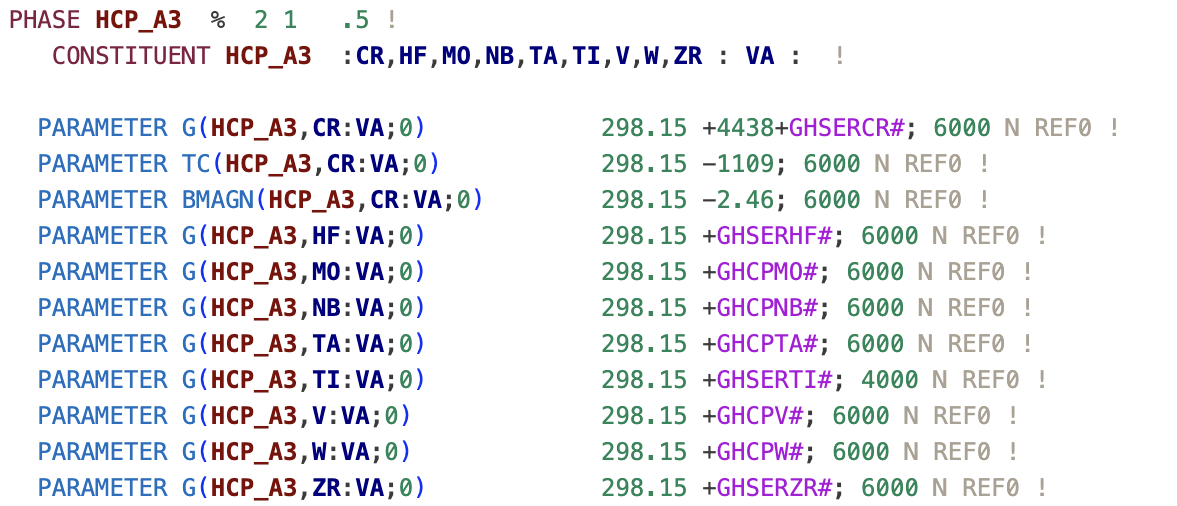
\includegraphics[width=0.65\textwidth]{tangentialsoft/Fig2-2.png}
    \caption{Thermodynamic parameter definitions in an example TDB file syntax-highlighted using \texttt{TDB-Highlighter}.}
    \label{osoft:fig:tdbfunctions}
\end{figure}

Furthermore, since the syntax-highlighting is not encoding colors, but rather tokens classifying TDB based on patterns, \texttt{TDB-Highlighter} works with any color scheme giving it improved customizability and accessibility. These include high-contrast schemes for people with poor vision, different types of color-blind schemes, or their dark versions, such as the one shown in Figure~\ref{osoft:fig:tdbdarkmode}.

\begin{figure}[H]
    \centering
    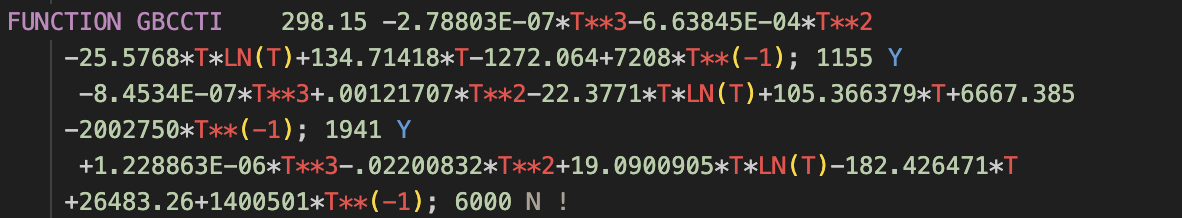
\includegraphics[width=0.65\textwidth]{tangentialsoft/Fig3.png}
    \caption{An example of \texttt{TDB-Highlighter} output under a "dark-mode" color scheme example.}
    \label{osoft:fig:tdbdarkmode}
\end{figure}

\hspace{24pt} 
\textit{Source available at:} 
\href{https://github.com/amkrajewski/TDB-Highlighter}{https://github.com/amkrajewski/TDB-Highlighter}



\section{\texttt{pymatgen.core} Contributions} \label{osoft:sec:pymatgen}

In addition to several discussion and bug reporting meta-contributions, two critical contributions to the \texttt{core} of \texttt{pymatgen} were made. One was an \emph{enhancement} to the \texttt{core.Composition} class enabling construction of these objects from weight fraction dictionaries, which was a long-missing feature needed by metallurgists and other scientists working with real/physical materials. The second one was a \emph{fix} of a bug in the \texttt{core.Composition} causing incompatibility with \texttt{OPTIMADE} due to incorrect calculations of the Hill formula.

\hspace{24pt} 
\textit{Source available at:} 
\href{https://github.com/materialsproject/pymatgen}{https://github.com/materialsproject/pymatgen}


\section{LLNL \texttt{MAP} Platform} \label{osoft:sec:map}

Exploration of the MPEA or HEA design space is a challenging task, partly due to the combinatorial intensity in composition. For non-equiatomic alloys with more than a few components, methods investigating a grid of compositions fail sooner or later depending on how fine the grid is.

\texttt{MAP} is an unreleased internal Lawrence Livermore National Lab high entropy alloy discovery platform, core of which has been designed from scratch by Adam M. Krajewski during MaCI and CCMS programs in Summer 2022 and Summer 2023 under Contract DE-AC52-07NA27344.

It implements a method of efficient searching for novel alloys that combines (1) highly optimized Black-Box Optimization (BBO) multi-stage investigation of individual alloy systems using CALPHAD modeling and surrogate models for targeting properties with (2) on-the-fly decisions on systems to investigate and resources to allocate to each. 

The developed toolset runs parallel across systems, allowing rapid calculations on high-performance computers (HPCs), and is agnostic of the surrogate models, thus can be quickly re-used to target any properties. Here, we demonstrate targeting high yield strength at elevated temperatures in 10-component refractory systems.


\section{\texttt{pqam-dparamhu2021}} \label{osoft:sec:dparam}

A Python binding library has been added to a community model for D Parameter prediction by Hu et al. 2021, originally written in R. In the process, the underlying model has been significantly re-written, without affecting its output values, to enable large scale predictions needed by \texttt{ULTERA} ecosystem. The resulting version is 10-1000x times faster depending on the task volume and machine.

\hspace{24pt} 
\textit{Source available at:} 
\href{https://github.com/amkrajewski/pqam-dparamhu2021}{https://github.com/amkrajewski/pqam-dparamhu2021}



\section{\texttt{pqam-rmsadtandoc2023}} \label{osoft:sec:rmsad}

A community model by Tandoc et al. 2023 designed for prediction of Root Mean Square Atomic Displacement (RMSAD) has been restructured as a PyQAlloyModel (\texttt{PQAM}) and trimmed down to provide minimal interface needed to run inference within the \texttt{ULTERA} ecosystem. In this dissertation, it is used later in Appendices \ref{chap:nimplextutorial1} and \ref{chap:nimplextutorial2} as a demonstrator property model.

\hspace{24pt} 
\textit{Source available at:} 
\href{https://github.com/amkrajewski/pqam-dparamhu2021}{https://github.com/amkrajewski/pqam-dparamhu2021}




\section{\texttt{MaterialsMap} Contributions} \label{osoft:sec:materialsmap}

\texttt{MaterialsMap} is an effort parallel to the \texttt{nimplex} which performs traditional community approach to similar problems but with much lower generality that enables application of more in-depth crafted methods.

\hspace{24pt} 
\textit{Source available at:} 
\href{https://github.com/PhasesResearchLab/MaterialsMap}{https://github.com/PhasesResearchLab/MaterialsMap}



\section{\texttt{MPDD-ALIGNN}} \label{osoft:sec:mpddalignn}

This fork of the \href{https://github.com/usnistgov/alignn}{JARVIS-ALIGNN} tool has been modified in several key ways to improve it towards \texttt{MPDD} and similar applications. 

\begin{itemize}
    \item A set of models of interest has been selected and defined in a \texttt{config.yaml} for consistency, readability, and easy tracking. These are the models which will be populating MPDD.
    \item \textbf{Dependency optimizations for running models}, skipping by default installation of several packages needed only for training and auxiliary tasks. Full set can still be installed by \texttt{pip install "mpdd-alignn[full]"}.
    \item The process of model fetching was reimplemented, making it similar to \texttt{pySIPFENN} by multi-threading connection to Figshare. Model \textbf{download is now 7 times faster}, fetching all 7 default models in 6.1 vs 41.4 seconds. Optimized what is included in the built package. Now, its \textbf{package size is reduced 33.5 times}, from 21.7MB to 0.65MB.
    \item Streamlined operation, where we can get results for a directory of POSCARS for all default models in just 3 quick lines.
    \begin{minted}[xleftmargin=3\parindent, linenos=true, fontsize=\small]{python}
    from alignn import pretrained
    pretrained.download_default_models()
    result = pretrained.run_models_from_directory(
      'example.SigmaPhase', mode='serial')
    \end{minted}
    which give a neat:
    \begin{minted}[xleftmargin=3\parindent, fontsize=\small, bgcolor=subtlegray]{output}
    [{
        'name': '9-Pb8O12.POSCAR',
        'ALIGNN-JARVIS Bulk Modulus [GPa]': 98.06883239746094,
        'ALIGNN-JARVIS Exfoliation Energy [meV/atom]': 101.71208190917969,
        'ALIGNN-JARVIS Formation Energy [eV/atom]': -1.1146986484527588,
        'ALIGNN-JARVIS MBJ Bandgap [eV]': 0.5845542550086975,
        'ALIGNN-JARVIS Shear Modulus [GPa]': 39.18968963623047,
        'ALIGNN-MP Formation Energy [eV/atom]': -1.4002774953842163,
        'ALIGNN-MP PBE Bandgap [eV]': 1.074204921722412
    },
    ...
    \end{minted}
\end{itemize}


\hspace{24pt} 
\textit{Source available at:} 
\href{https://github.com/amkrajewski/mpdd-alignn}{https://github.com/amkrajewski/mpdd-alignn}


\section{\texttt{spgnim}} \label{osoft:sec:spgnim}

\texttt{spgnim} is a \texttt{nim} library built around the state-of-the-art symmetry analysis \texttt{spglib} C library (\href{https://github.com/spglib/spglib}{https://github.com/spglib/spglib}) with the goals of (1) streamlining and optimizing internal calls for improved performance, (2) easy-to-use interface for non-C programmers, and (3) future interfacing with low-level \texttt{nim}-based atomistic featurization methods for \texttt{pySIPFENN}.

\hspace{24pt} 
\textit{Source available at:} 
\href{https://github.com/amkrajewski/spgnim}{https://github.com/amkrajewski/spgnim}



 
